\appendix

\chapter{Reproducibility}

\section{Implementation Details}
Here is a list of useful details regarding our implementation:
\begin{itemize}
    \item Python 3.12.7
    \item Anaconda virtual environment
    \item compressAI 1.2.6
    \item Code hosted on private GitHub repository
    \item Processing power provided by Télécom Paris GPU cluster (\url{https://docs.google.com/document/d/1lXykfpEUJCrbNh22D2f2kxNS0gV6t-j9A_juWFdiEnI/edit?tab=t.0})
\end{itemize}

\section{Measures}

% TODO

\chapter{Figures}

\begin{figure}
    \centering
    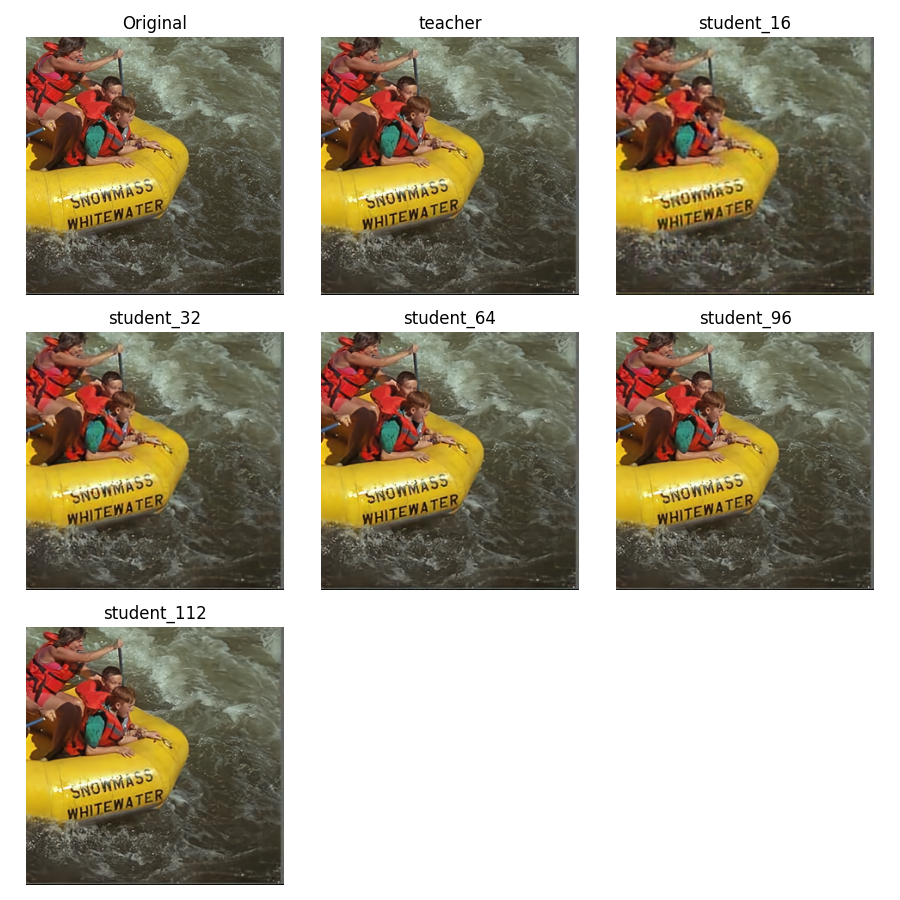
\includegraphics[width=15cm]{img/kd_ae_kodak_14.png}
    \caption[Evaluation on the Kodak dataset of the scale hyperprior student models trained for image compression: reconstruction results on image 14 of the Kodak dataset with teacher and student architectures.]{Evaluation on the Kodak dataset of the scale hyperprior student models trained for image compression: reconstruction results on image 14 of the Kodak dataset with teacher and student architectures.}
    \label{appendix:kd_ae_1}
\end{figure}

\begin{figure}
    \centering
    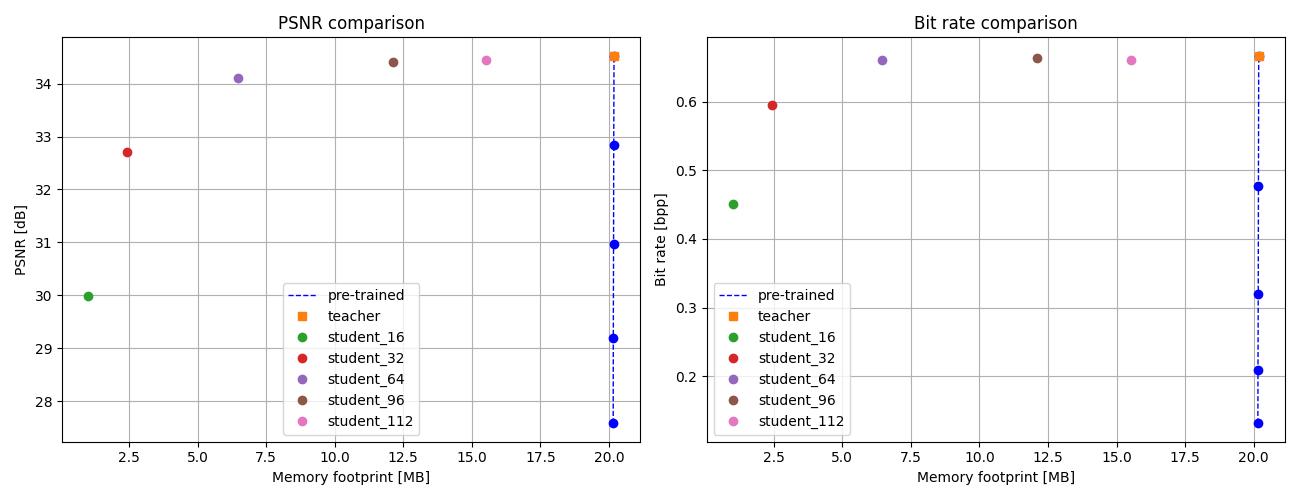
\includegraphics[width=15cm]{img/kd_lic_memory.png}
    \caption[\acrshort{psnr} and bit rate on the Kodak dataset according to students memory footprint.]{\acrshort{psnr} and bit rate on the Kodak dataset according to students memory footprint.}
    \label{appendix:kd_lic_memory}
\end{figure}

\begin{figure}
    \centering
    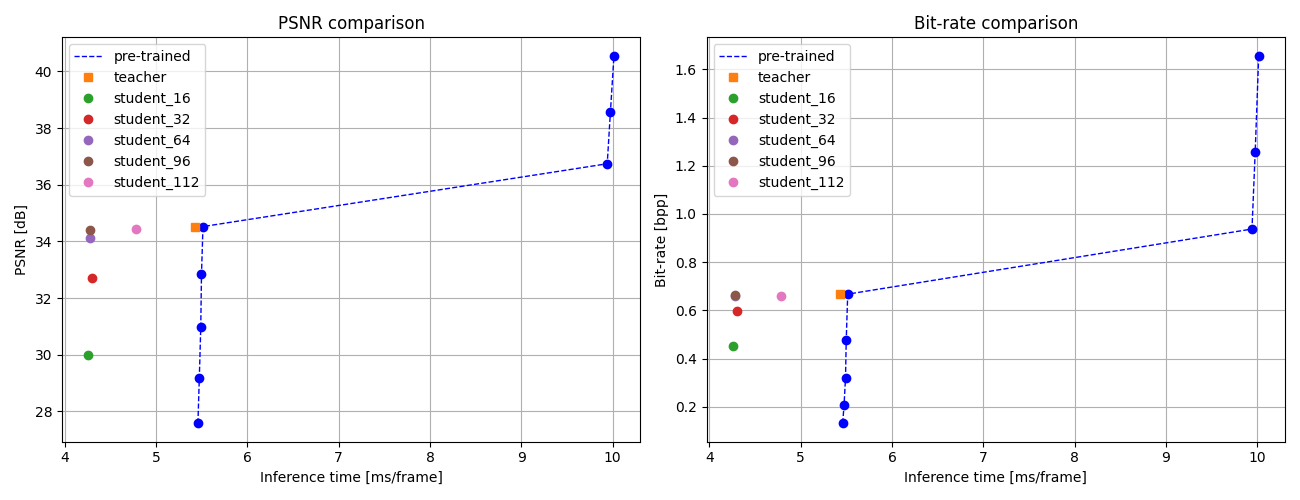
\includegraphics[width=15cm]{img/kd_lic_time.png}
    \caption[\acrshort{psnr} and bit rate on the Kodak dataset according to students inference time.]{\acrshort{psnr} and bit rate on the Kodak dataset according to students inference time.}
    \label{appendix:kd_lic_time}
\end{figure}

\begin{sidewaystable}[]
    \centering
    \begin{tabular}{|c|c|lr|lr|lr|lr|lr|lr|lr|}
        \hline
        Model                     & \begin{tabular}[c]{@{}c@{}}Number\\ of channels\end{tabular} & \multicolumn{2}{c|}{\begin{tabular}[c]{@{}c@{}}Number of\\ parameters {[}M{]}\end{tabular}} & \multicolumn{2}{c|}{\begin{tabular}[c]{@{}c@{}}Memory\\ footprint {[}MB{]}\end{tabular}} & \multicolumn{2}{c|}{\begin{tabular}[c]{@{}c@{}}Floating point\\ operations\\ {[}GFLOP/frame{]}\end{tabular}} & \multicolumn{2}{c|}{\begin{tabular}[c]{@{}c@{}}Throughput\\ {[}FPS{]}\end{tabular}} & \multicolumn{2}{c|}{\begin{tabular}[c]{@{}c@{}}Energy\\ {[}mJ/frame{]}\end{tabular}} & \multicolumn{2}{c|}{PSNR}               & \multicolumn{2}{c|}{\begin{tabular}[c]{@{}c@{}}Bit rate\\ {[}bpp{]}\end{tabular}}      \\ \hline
        Teacher                   & 128                        & {\color[HTML]{656565} }                                  & 5.08                         & {\color[HTML]{656565} }                                  & 20.18                        & {\color[HTML]{656565} }                                  & 34.24                        & {\color[HTML]{656565} }                                  & 184.20                         & {\color[HTML]{656565} }                                  & 1767.85                         & {\color[HTML]{656565} }                                 & 34.53                         & {\color[HTML]{656565} }                                 & 0.67                         \\ \hline
                                  & 112                        & {\color[HTML]{656565} -19.77 \%}                         & 4.07                         & {\color[HTML]{656565} -23.03 \%}                         & 15.53                        & {\color[HTML]{656565} -22.01 \%}                         & 26.70                        & {\color[HTML]{656565} +13.47 \%}                         & 209.01                         & {\color[HTML]{656565} -9.47 \%}                          & 1600.41                         & {\color[HTML]{656565} -0.26 \%}                         & 34.44                         & {\color[HTML]{656565} -1.03 \%}                         & 0.66                         \\ \cline{2-16} 
                                  & 96                         & {\color[HTML]{656565} -37.47 \%}                         & 3.17                         & {\color[HTML]{656565} -40.01 \%}                         & 12.11                        & {\color[HTML]{656565} -41.31 \%}                         & 20.10                        & {\color[HTML]{656565} +25.74 \%}                         & 231.61                         & {\color[HTML]{656565} -19.88 \%}                         & 1416.34                         & {\color[HTML]{656565} -0.33 \%}                         & 34.41                         & {\color[HTML]{656565} -0.58 \%}                         & 0.66                         \\ \cline{2-16} 
                                  & \cellcolor[HTML]{EFEFEF}64 & \cellcolor[HTML]{EFEFEF}{\color[HTML]{656565} -66.62 \%} & \cellcolor[HTML]{EFEFEF}1.69 & \cellcolor[HTML]{EFEFEF}{\color[HTML]{656565} -67.98 \%} & \cellcolor[HTML]{EFEFEF}6.46 & \cellcolor[HTML]{EFEFEF}{\color[HTML]{656565} -71.75 \%} & \cellcolor[HTML]{EFEFEF}9.67 & \cellcolor[HTML]{EFEFEF}{\color[HTML]{656565} +26.20 \%} & \cellcolor[HTML]{EFEFEF}232.47 & \cellcolor[HTML]{EFEFEF}{\color[HTML]{656565} -34.15 \%} & \cellcolor[HTML]{EFEFEF}1164.17 & \cellcolor[HTML]{EFEFEF}{\color[HTML]{656565} -1.21 \%} & \cellcolor[HTML]{EFEFEF}34.11 & \cellcolor[HTML]{EFEFEF}{\color[HTML]{656565} -0.91 \%} & \cellcolor[HTML]{EFEFEF}0.66 \\ \cline{2-16} 
                                  & 32                         & {\color[HTML]{656565} -87.46 \%}                         & 0.64                         & {\color[HTML]{656565} -87.97 \%}                         & 2.43                         & {\color[HTML]{656565} -91.31 \%}                         & 2.98                         & {\color[HTML]{656565} +25.89 \%}                         & 231.90                         & {\color[HTML]{656565} -60.45 \%}                         & 699.18                          & {\color[HTML]{656565} -5.25 \%}                         & 32.71                         & {\color[HTML]{656565} -10.73 \%}                        & 0.60                         \\ \cline{2-16} 
        \multirow{-5}{*}{Student} & 16                         & {\color[HTML]{656565} -94.77 \%}                         & 0.27                         & {\color[HTML]{656565} -94.98 \%}                         & 1.01                         & {\color[HTML]{656565} -97.01 \%}                         & 1.02                         & {\color[HTML]{656565} +26.83 \%}                         & 233.63                         & {\color[HTML]{656565} -61.28 \%}                         & 684.45                          & {\color[HTML]{656565} -13.17 \%}                        & 29.98                         & {\color[HTML]{656565} -32.44 \%}                        & 0.45                         \\ \hline
    \end{tabular}
    \caption{}
    \label{appendix:tab_resources}
\end{sidewaystable}